
\documentclass[10pt]{article}
\usepackage{color}
\usepackage{makeidx}
\usepackage{graphicx}
\usepackage{underscore}
\usepackage{enumitem}
\usepackage{pdfpages}
\newlist{longenum}{enumerate}{5}
\setlist[longenum,1]{label=\roman*)}
\setlist[longenum,2]{label=\alph*)}
\setlist[longenum,3]{label=\arabic*)}
\setlist[longenum,4]{label=(\roman*)}
\setlist[longenum,5]{label=(\alph*)}
\usepackage[section]{placeins}
\makeindex
\begin{document}
\begin{titlepage}
\centering
\huge{CMPE 315: Principles of VLSI Design Project Cover Page}
\vfill
\flushleft
\large{
Final Project\\
}
\vfill
Name: Brian Weber\\
Section: CMPE640 01\\
\vfill
Date Submitted: 11/22/2017
\vfill
\Large{TA / Grader Use Only:}\\
Late Submission Deduction (20\% per day):\\
\vspace{1cm}
Other Deductions:\\
\vspace{3cm}
Final Lab Grade:\\
\vspace{1cm}
Comments to student:\\
\vspace{5cm}
\end{titlepage}
\tableofcontents
    \section{Current Status of Code (Read Me)}
        Before getting into the bulk of the report I would like to write a short
summary of the status of my code. Based on my tests, everything works
completely, and every layout LVS matches. Every entity that a layout was made
for was optimized slightly for CMOS. State machine modules are still suboptimal,
but work.
\section{Entity Hierarchy}
    All entities are paired with architecture "structural".
    \begin{longenum}
    \item chip
        \begin{longenum}
        \item Counter
            \begin{longenum}
            \item rd_wr_hit_miss_reg
                \begin{longenum}
                \item dff_reset
                \item{Dlatch_Reset}
                \end{longenum}
            \item SR18
                \begin{longenum}
                \item dff_reset_high
                \end{longenum}
            \item dff_reset_high
            \item dff_reset
            \item srff
            \end{longenum}
        \item Cache_Block
            \begin{longenum}
            \item Cache_Cell_Row
                \begin{longenum}
                \item Cache_Cell_Valid
                    \begin{longenum}
                    \item SRlatch
                    \item tx
                    \end{longenum}
                \item Cache_Cell_Tag
                    \begin{longenum}    
                    \item Cache_Cell
                    \end{longenum}
                \item Cache_Cell_Data_Block
                    \begin{longenum}
                    \item Cache_Cell
                    \end{longenum}
                \end{longenum}
            \end{longenum}
        \item Decoder
        \item Hit_Miss
            \begin{longenum}
            \item Compare
            \end{longenum}
        \item Output_Enable
            \begin{longenum}
            \item tx
            \end{longenum}
        \item register8
            \begin{longenum}
            \item dff_reset
            \end{longenum}
        \end{longenum}
    \end{longenum}
\section{Chip}
    For the most part, this design sticks to the overall design shown in the
prompt. However, this design only uses one decoder to select which cache cell
will be operated on, rather than both a decoder and a multiplexor. The chip
functions as follows. A read miss will take 19 clocks to complete. A read hit
will take 19 clock cycles from the beginning of the busy signal, to when the
cache stops outputting data. A read hit will take 2, and write hits and misses
take 3. On a read miss, on the second clock cycle, the cache will enable the
memory, and pass on the adress from the cpu. 7 clock cycles after enable goes
low, the data will arrive on the memory data input. The cache gets 2 cycles to
save the data, before the next value from the word of memory arrives. After all
four values are written, the cache waits one more clock cycle before outputting
the data that was asked for by the cpu. This process can be seen in Figure
\ref{chiprm}. On a read hit, busy stays high for one clock before going low, and
outputting the data. This process can be seen in \ref{chiprh}. On write miss,
busy goes high for 2 cycles before going low. No data is read or edited. On a
write hit, busy stays high for 2 cycles. The new value is written to the cache,
and the new value should be available one cycle after busy goes low. Figures
\ref{chipwm} and \ref{chipwh} show a write miss and a write hit respectively. An
overall view of the chip is shown in Figure \ref{chiphd}.

I placed a lot of my logic that decides what and when to write within the
Cache_Cells and rows. This increases size, but simplifies design as the output
of the logic will have a much lower fanout, and therefore lower load. This
allowed me to not need to worry about parasitic capacitances as much. 

\begin{figure}
    \centering
    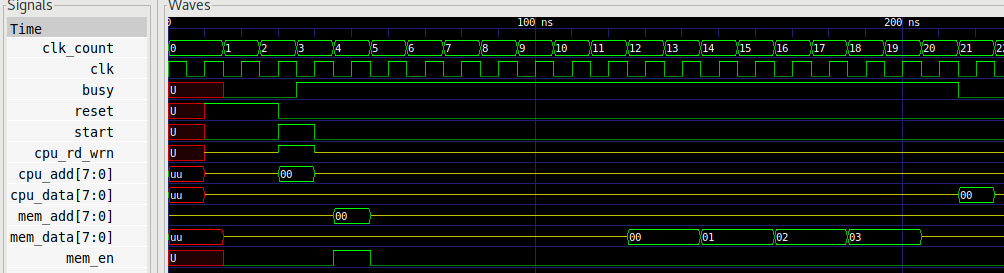
\includegraphics[width=\textwidth]{chiprm.png}
    \caption{Timing of read miss.}
    \label{chiprm}
\end{figure}

\begin{figure}
    \centering
    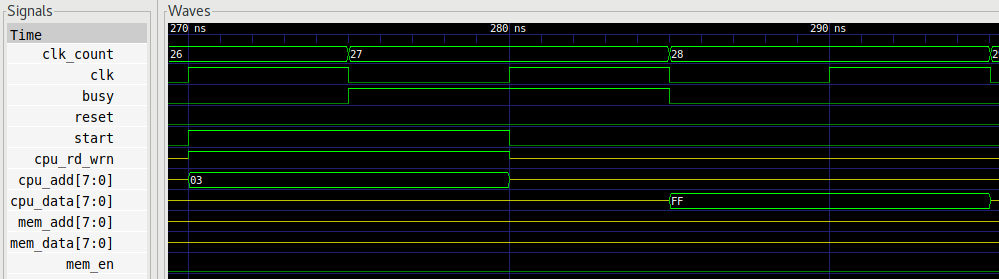
\includegraphics[width=\textwidth]{chiprh.png}
    \caption{Timing of read hit.}
    \label{chiprh}
\end{figure}
\begin{figure}
    \centering
    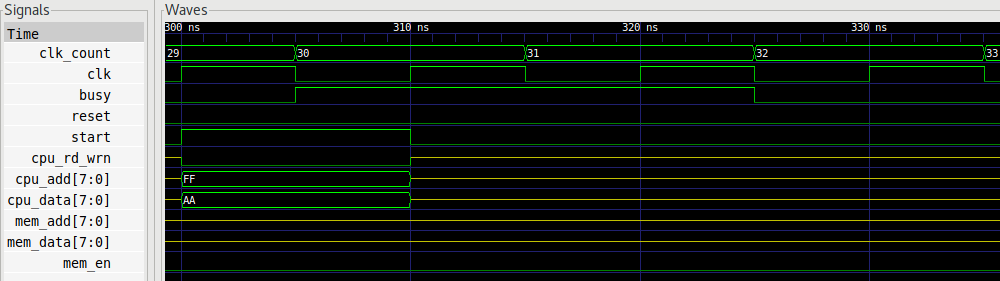
\includegraphics[width=\textwidth]{chipwm.png}
    \caption{Timing of write miss.}
    \label{chipwm}
\end{figure}
\begin{figure}
    \centering
    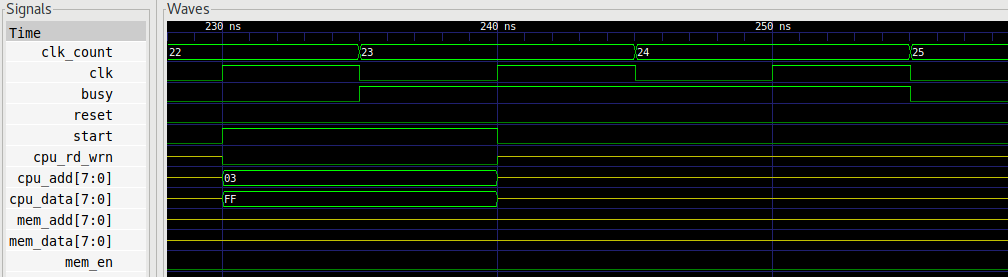
\includegraphics[width=\textwidth]{chipwh.png}
    \caption{Timing of write hit.}
    \label{chipwh}
\end{figure}

\begin{figure}
    \centering
    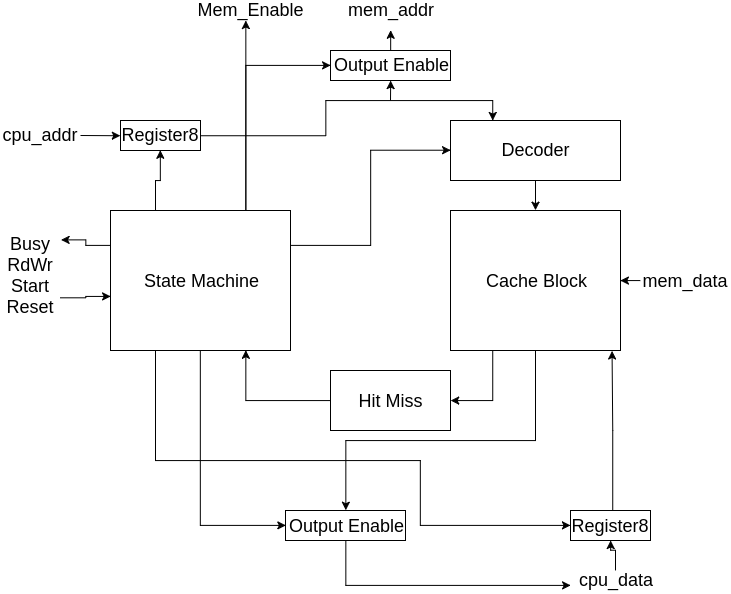
\includegraphics[width=\textwidth]{chd.png}
    \caption{A high level view of the chip module.}
    \label{chiphd}
\end{figure}

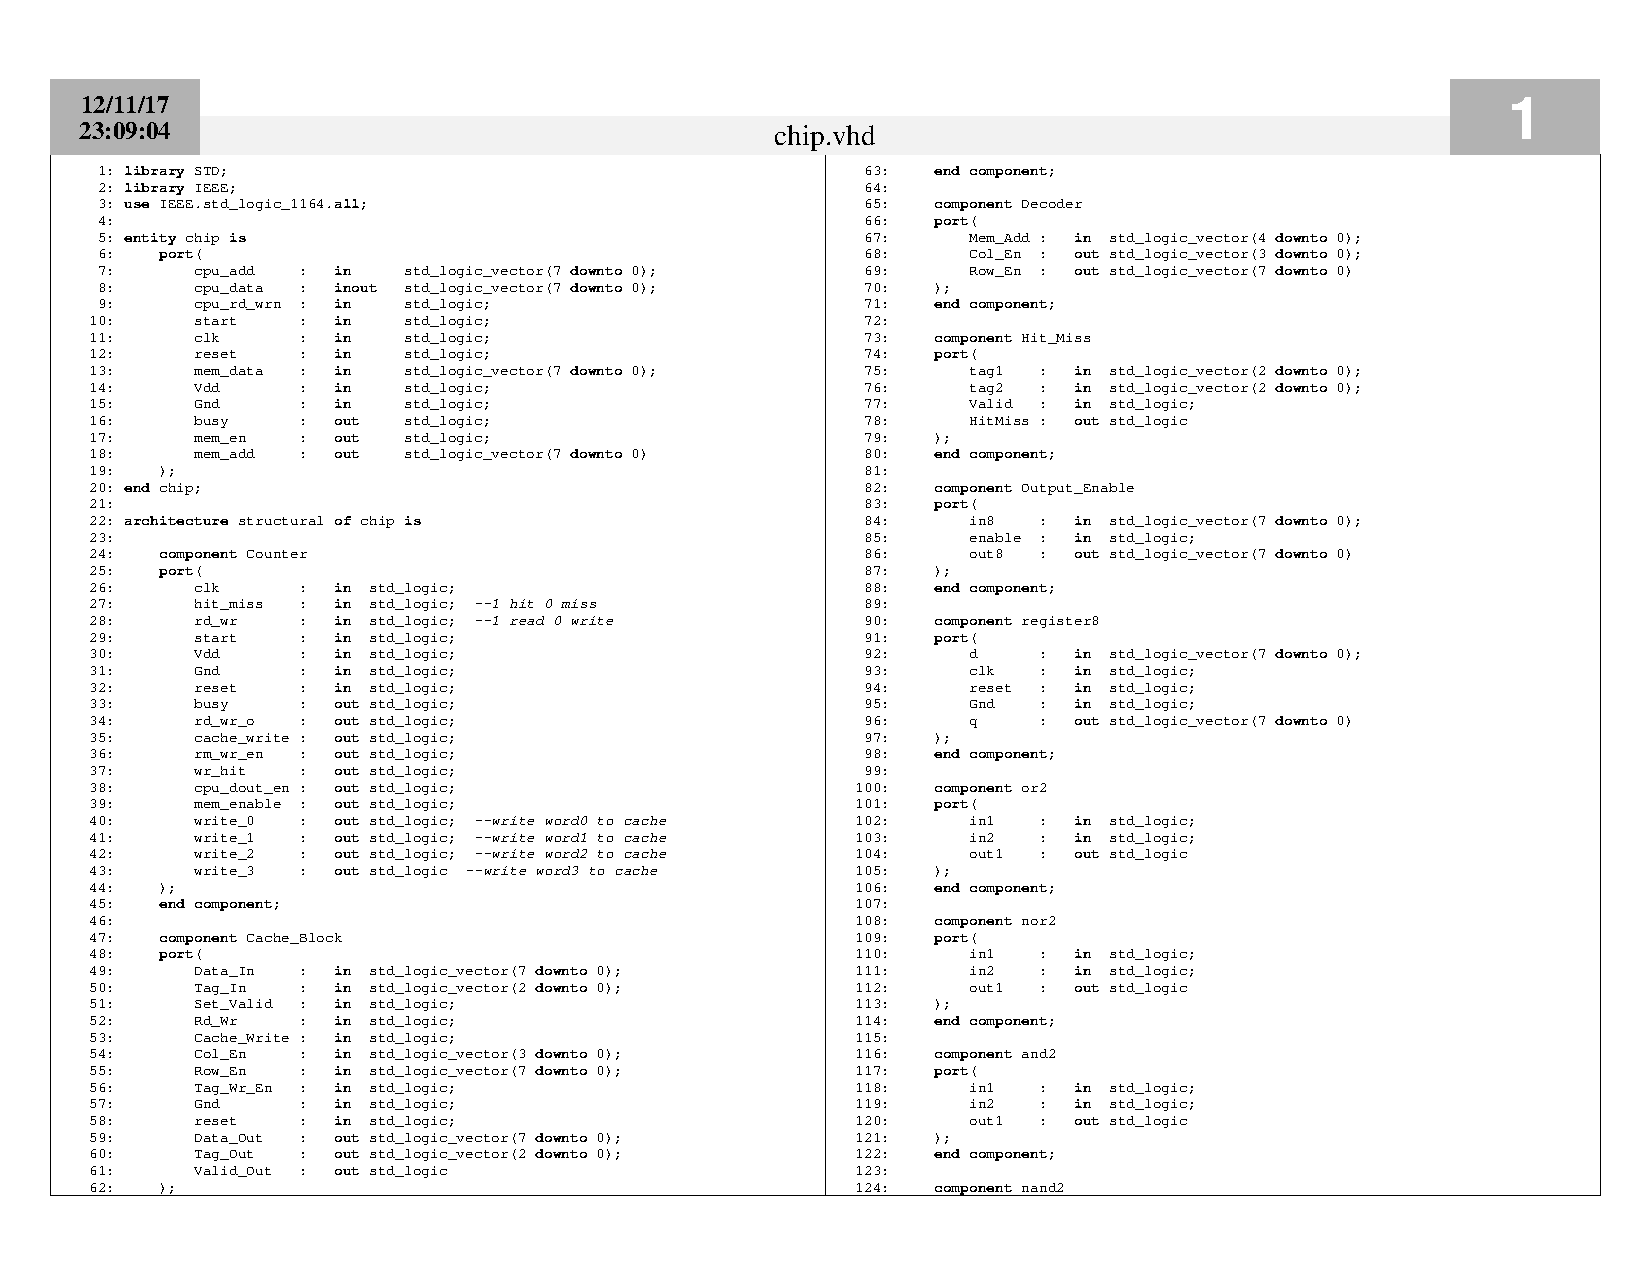
\includepdf[pages=-, landscape=true]{chip.pdf}
\newpage
\newpage
\section{Counter (State Machine)}
        The state machine is an entity called Counter, which is centered around
a shift register that keeps track of the number of clocks that pass after the
busy signal goes high. Depending on hit/miss status of each operation, different
things are done depending on the clock count after busy is set high. Another key
part of the state machine is a group of registers for storing both the inputs
from the cpu, and whether or not there was a hit or a miss. There is an entity
called rd_wr_hit_miss_reg that stores the operation (rd or write), as well as
whether it was a hit or miss, and outputs 4 separate lines. Figures
\ref{crdmiss}, \ref{crdhit}, \ref{cwrmiss}, and \ref{cwrhit} show input and
output waveforms that were generated from the test bench Counter_Test. Figure
\ref{sd} shows a state diagram of the state machine. Figure \ref{state} shows
the high level view of the hierarchy of the state machine. These waveform figures
prove the correct operation of the state machine. The definitions of the signals
are as follows:
\begin{itemize}
    \item s_reset: (Input) The global reset signal.
    \item s_clk: (Input) The global clock signal.
    \item s_busy: (Output) The global busy signal.
    \item s_start: (Input) The start signal from the CPU.
    \item s_cpu_dout_en: (Output) The signal which enables the transmission gate
from cache output to the CPU.
    \item s_cache_write: (Output) The signal which triggers all writes to the
cache. It is connected to the cache block.
    \item s_hit_miss: (Input) The signal from the Hit_Miss module indicating whether
there is a hit or a miss.
    \item s_mem_enable: (Output) The signal that enables external memory.
    \item s_rd_wr: (Input) The rd_wr signal given from the CPU.
    \item s_rd_wr_o: (Output) A rd_wr signal that is sent to other modules after
the original rd_wr is latched.
    \item s_rm_wr_en: (Output) A signal that allows writing to the cache during
a read miss.
    \item s_wr_hit: (Output) A signal that is sent to other modules so they know
there was a write hit.
    \item s_write_[0:3]: (Output) Signals that select which block to be written
to during read a read miss. When used with s_rm_wr_en, they override the which
column the decoder is currently selecting.
\end{itemize} 

\begin{figure}[!htb]
    \centering
    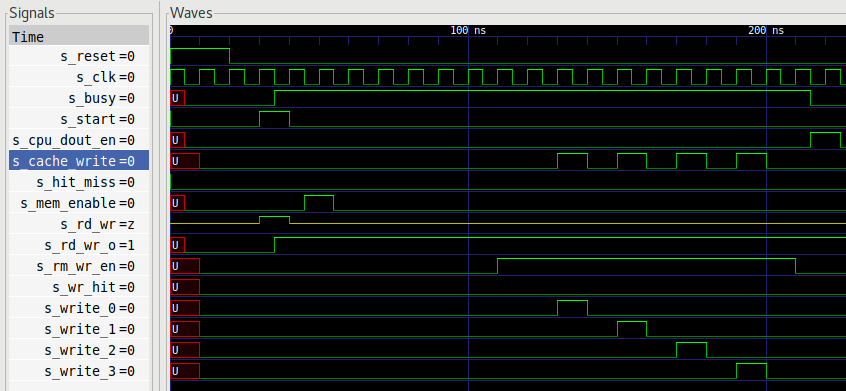
\includegraphics[width=\textwidth]{crm.png}
    \caption{Counter module timing during read miss.}
    \label{crdmiss}
\end{figure}

\begin{figure}[!htb]
    \centering
    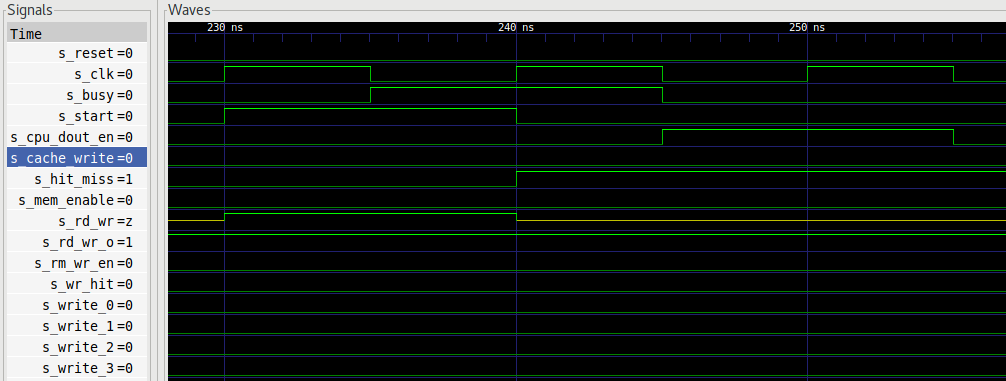
\includegraphics[width=\textwidth]{crh.png}
    \caption{Counter module timing during read hit.}
    \label{crdhit}
\end{figure}

\begin{figure}[!htb]
    \centering
    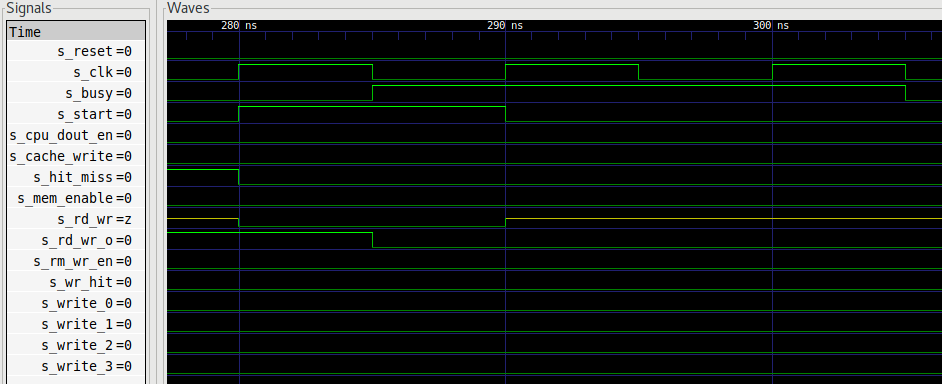
\includegraphics[width=\textwidth]{cwm.png}
    \caption{Counter module timing during write miss.}
    \label{cwrmiss}
\end{figure}

\begin{figure}[!htb]
    \centering
    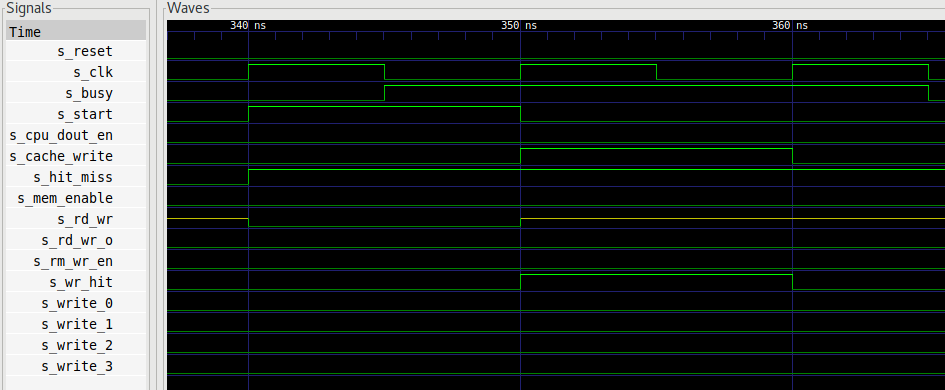
\includegraphics[width=\textwidth]{cwh.png}
    \caption{Counter module timing during write hit.}
    \label{cwrhit}
\end{figure}

\begin{figure}[!htb]
    \centering
    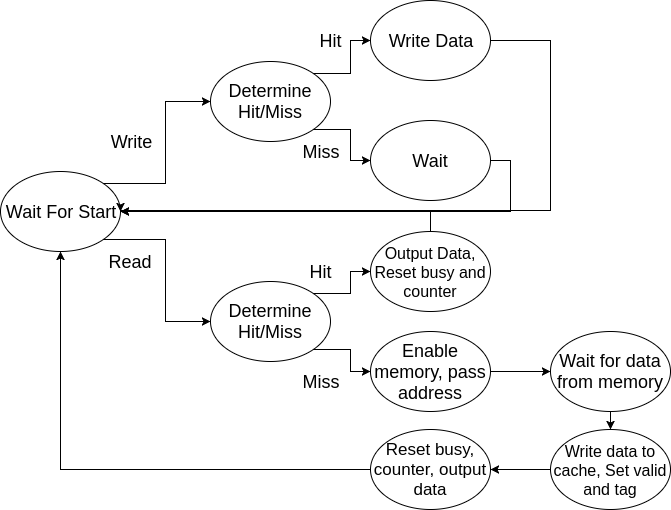
\includegraphics[width=\textwidth]{sd.png}
    \caption{State diagram of the state machine.}
    \label{sd}
\end{figure}

\begin{figure}[!htb]
    \centering
    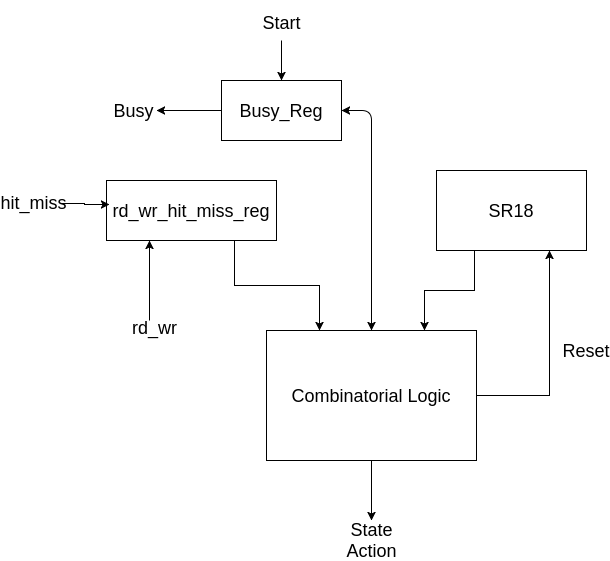
\includegraphics[width=\textwidth]{state.png}
    \caption{High level view of state machine hierarchy.}
    \label{state}
\end{figure}

\subsection{rd_wr_hit_miss_reg}
This module is responsible for storing the state of rd_wr, and hit_miss, as well
as generating signals for the current combination. During operation, first rd_wr
is stored, then once hit_miss is ready, that is latched as well. The rd_wr value
is stored in a D flip flop, and the hit_miss value is stored in a D Latch. There
are other inputs and logic to enable the clock and latch of each. It then uses
some simple logic to generate individual signals for each possible combination
of rd_wr and hit_miss. As Figure \ref{rwhm} shows, after both, rd_wr and
hit_miss are set high, read_hit is set high.

\begin{figure}
    \centering
    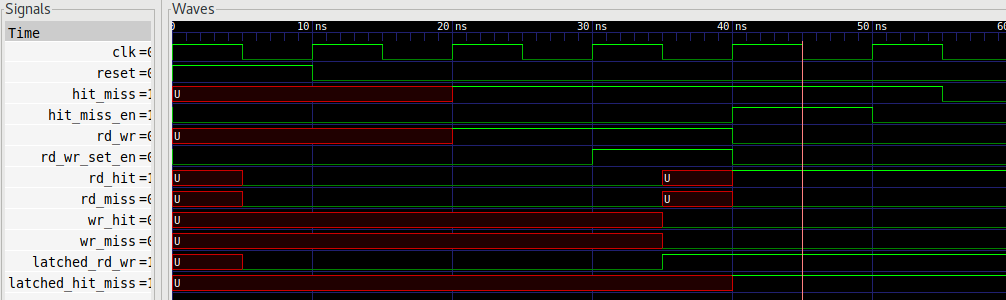
\includegraphics[width=\textwidth]{rwhm.png}
    \caption{Functionality of the rd_wr_hit_miss_reg module.}
    \label{rwhm}
\end{figure}

\subsection{SR18}
This module is just a simple shift register to keep track of how long the busy
signal is high. Using this, the rd_wr_hit_miss_reg, and some combinational
logic, it is relatively easy to determine when certain actions have to be
performed. Figure \ref{sr18} shows how this module counts clocks.

\begin{figure}
    \centering
    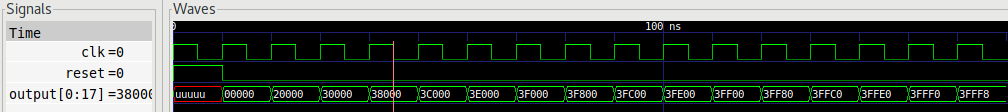
\includegraphics[width=\textwidth]{sr18.png}
    \caption{The SR18 module counting clock cycles.}
    \label{sr18}
\end{figure}

\section{Cache_Block}
The cache block is a block of positive latch enabled Dlatches, indexed by the
cpu address. In front of each Dlatch is a transmission gate. The inputs and
outputs of each row all come from and lead to the same 8 bit bus, but only one row at a time can
be selected due to the Decoder module. This prevents conflicts on the outputs as
well as prevents more than one row from being written to at a time. The valid
cells are asynchronous sr latches, and are set while data is being written from
memory during a read miss. Tags are also set at this time. The valid and tag
bits are output as soon as a row is selected, however, for a byte to be
output, the internal rd_wr signal must be high, and a column must be selected.
The Cache_Block was split into several modules for  convenience. First it is
split into rows, called Cache_Cell_Row. The rows are split into 4 8 bit data
blocks, called Cache_Cell_Data_Block, a tag block called Cache_Cell_Tag, and a
valid bit, called Cache_Cell_Valid. The Valid bit is an sr latch, while the the
tag and data blocks are made up of 3 and 8 individual bit modules called
Cache_Cell. This Cache_Cell is a resettable Dlatch with a transmission gate in
front for enabling output. Figure \ref{cb} shows a waveform diagram of the cache
block. At 10 ns, the data arrives at the input, the rd signal is turned on, and
the row and column are selected. At 15 ns, cache_write is turned on, writing the
input data. Since rd is on, the data shows on the output as well. At 15 ns, the
tag and valid bits are also set. Notice that after the rd signal turns off at 20
ns, the data output becomes high impedence, however the tag and valid bits
continue to output. At 30 ns, different data is set at a different position. At
40 ns, the old data is read, and at 45 ns, the new data is read. Here is a
description of all the signals:
\begin{itemize}
    \item data_in: (Input) Input data to the cache.
    \item data_out: (Output) Output data from the cache.
    \item rd_wr: (Input) Internal read write signal used for enabling data
output.
    \item cache_write: (Input) Signal used to trigger writing of data to cache.
    \item row_en: (Input) Signal used for selecting which row to operate on.
    \item col_en: (Input) Signal used for selecting which column to operate on.
    \item tag_out: (Output) Output of tag of selected row.
    \item tag_in: (Input) Input tag to the cache.
    \item tag_wr_en: (Input) Triggers writing the tag to the row.
    \item set_valid: (Input) Sets the valid sr latch on the selected row.
    \item valid_out: (Output) Output of the selected row's valid bit.
    \item reset: (Input) Global reset.
\end{itemize}
\begin{figure}[!htb]
    \centering
    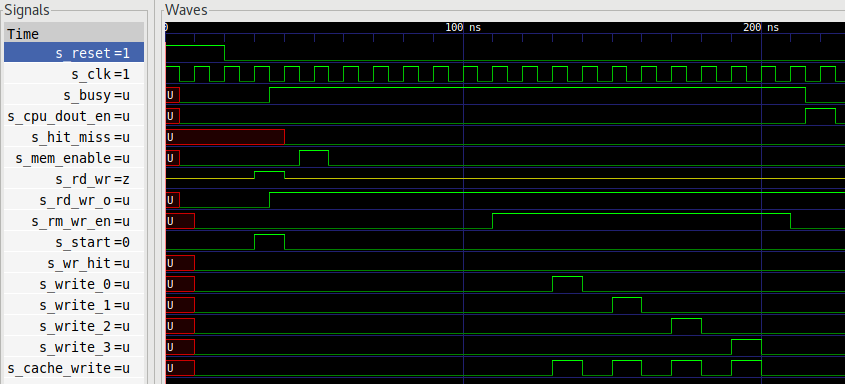
\includegraphics[width=\textwidth]{cb.png}
    \caption{Timing diagram showing the functionality of the cache_block.}
    \label{cb}
\end{figure}
\section{Decoder}
The decoder selects which byte operations are to be performed on based on the
memory address. It does this asynchronously. It still has to be optimized for
cmos. Only one bit of each output is turned on at a time. The first Three bits
of input index the row, and the last 2 index the column. Figure \ref{d} shows
example inputs and outputs.  
\begin{figure}[!htb] 
    \centering
    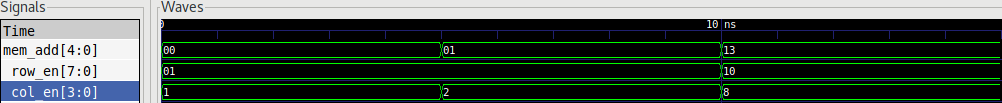
\includegraphics[width=\textwidth]{d.png}
    \caption{Functionality of the decoder module.}
    \label{d}
\end{figure}
\section{Hit Miss}
This module is responsible for determining if there is a hit or a miss, based on
the tag from the cache, and the tag from the memory address, as well as the
valid bit from the selected row of the cache. There is a hit if both the tags
match, and the valid bit is high. This module is asynchronous as well, and
because the value of its output may change as the cache is written to (even
within the same operation), its initial value is latched within the state
machine in the beginning of each operation. There is a module called compare
inside Hit_Miss which is reponsible for deterining whether the tags are
equivalent. Figure \ref{hm} shows example inputs and outputs of this module.
\begin{figure}[!htb]
    \centering
    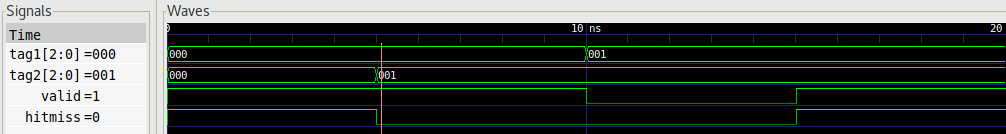
\includegraphics[width=\textwidth]{hm.png}
    \caption{Functionality fo the Hit_Miss module.}
    \label{hm}
\end{figure}
\section{Register8 and OutputEnable}
These two modules are used to control IO to the cpu and memory. The registers
ave the data that is sent from the cpu, and the Output_Enable module is used to
mask output to the data bus until it is needed. The register8 module uses an
array of negative edge trigger D flip flops, and the Output_Enable module uses
an array of 8 transmission gates.
\end{document}
